% Requires running Bibtex

\documentclass[%
reprint,
amsmath,amssymb,
aps,
]{revtex4-2}

\usepackage{graphicx}% Include figure files
\usepackage{dcolumn}% Align table columns on decimal point
\usepackage{bm}% bold math
\usepackage{hyperref}% add hypertext capabilities
\usepackage[font=scriptsize,labelfont=bf, justification=justified]{caption}% change fontsize in captions
\usepackage{booktabs}% cool table style
\hypersetup{
	colorlinks=true,       % false: boxed links; true: colored links
	linkcolor=black,        % color of internal links
	citecolor=black,        % color of links to bibliography
	filecolor=black,     % color of file links
	urlcolor=black         
}

\usepackage{bibspacing}
\setlength{\bibitemsep}{.5\baselineskip plus .05\baselineskip minus .05\baselineskip}


\begin{document}
	
	\preprint{APS/123-QED}
	
	\title{PHYC30170 Physics with Astronomy and Space Science Lab 1;\\An Investigation of Surface Plasmon Resonance}
	
	\author{Daragh Hollman}
	\email{daragh.hollman@ucdconnect.ie}
	
	\date{\today}
	
	\begin{abstract}
		The aims of this experiment were to determine the excitation angle of the surface plasmon within the Kretschmann configuration and to investigate the dependence of surface plasmon resonance (SPR) on the wavelength of the incident light and the thickness of the silver foil. [NOT FINISHED]
	\end{abstract}

	\maketitle
	
	\section{Introduction}		
		Surface plasmons are transverse magnetic waves, comprised of oscillating electrons, which travel along the boundary of a metal and a dielectric \cite{undergradToledo}. They were first discovered in 1957 by R. H. Ritchie The study of surface plasmons is very important and has many applications in biophysics, particularly in the analysis of biomolecular interactions \cite{biomedicalApplications}, and in many fields of optics including but not limited to sub-wavelength optics and near-field optics \cite{opticalApplications}.
	
	\section{Theory}
		\subsection{Excitation of Free Electrons}
			\url{https://iopscience-iop-org.ucd.idm.oclc.org/article/10.1088/0022-3727/45/11/113001}
		
		\subsection{Surface Plasmon Waves}
		
			Mention polariton
		
		\subsection{Apparatus}
			The apparatus was set up as shown in figure \ref{fig:apparatus}. More specifically, the Kretschmann configuration was used, figure \ref{fig:kConfig}.
			
			
			Describe the prism
			
			External vs internal angle
			\begin{figure}
				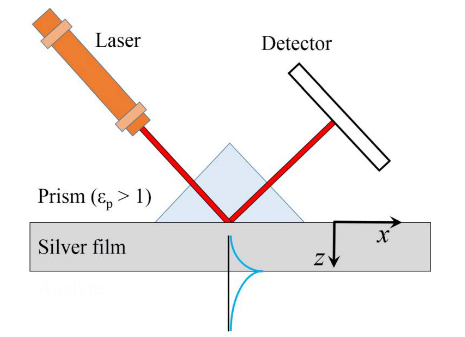
\includegraphics[width=0.9\columnwidth]{kConfig.png}
				\caption{\label{fig:kConfig}The Kretschmann configuration. The silver film was evaporated onto the glass prism. The light from the laser excites the electrons and a surface plasmon polariton is formed on the outer side of the film. \cite{opticalApplications}}
			\end{figure}
		
			\begin{figure}
				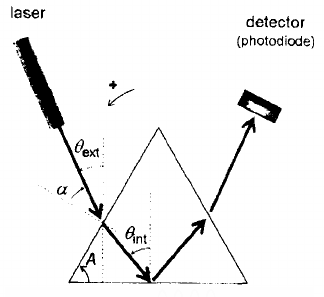
\includegraphics[width=0.7\columnwidth]{anglesDiagram.png}
				\caption{\label{fig:angles}A diagram describing the external and internal angles \cite{pluchery}.}
			\end{figure}
	 
	\section{Methodology}
		\subsection{Apparatus Setup}
			The apparatus was set up in the Kretschmann configuration as shown in figure \ref{fig:kConfig}. A silver film was evaporated onto three prisms so that the thickness of the film could be varied. Thicknesses of 10nm, 13nm, and 15nm were used. The prism was placed in the centre of a bidirectional stepping rotary table. This table had two independently movable discs (specifically one disc and one annulus) controlled by stepper motors which, through a gear system, had a precision calibrated to be $0.045$ degrees per step. The prism was placed on the inner disc and a photodiode was fixed on the outer annulus to be used as a detector.\\
			
			The apparatus was controlled using Python 3 to interface with a USB multifunction I/O device, NI USB-6009 \cite{nationalInstruments}. This was used as a digital to analogue converter to control the stepper motors as well as an input from the photodiode to read voltages. A laser was placed into a retort stand such that it would pass through the prism and reflect off the silver film into the photodiode.

			\subsubsection{Light Source}
				Three He-Ne lasers were used of wavelengths 633nm, 515nm, and 405nm all of which had a maximum power $\le 4 \,\text{mW}$. In this report we will refer to these lasers as red, green, and blue respectively. A linear polarising filter was positioned between the laser and the prism such to p-polarise the incident light.
			
			\subsubsection{Motor Programming}
				The stepper motor modules were programmed following the documentation provided by UCD \cite{motorDoc}. They were controlled by digital signals to the control lines of the USB I/O device. The control lines were used to enable and disable the motors, set the direction, and to advance each motor. We initially had issues getting these inputs to work as one of the pins was wired incorrectly, however through exhaustive testing we were able to identify the correct pins for each input. A function was then written in Python to control the movement of these motors. This function took inputs of a number of steps, a direction, and a delay time. It was important to include a short delay ($\approx 100\,\text{ms}$) between steps to reduce unwanted vibrational artefacts in the data and to not overheat the motors. Functionality was also included to select to rotate either the prism, or the detector, or both. This function is included in appendix A.1 on data acquisition.
			
			\subsubsection{Developing an Algorithm for Data Collection}
				This function was then edited to include capabilities to include data collection from the photodiode while moving. After each step 100 samples of the voltage were taken at $10,000\,\text{Hz}$. The mean of these was recorded as the voltage value and the standard deviation was taken as the uncertainty.\\
				
				To improve efficiency, functionality to drive the system backwards as well as forwards was introduced to remove the time taken to reset the apparatus to its initial position.\\
				
				Note that the detector had to move twice for every prism step to keep the laser tracked on the detector. This was due to their separation.

			\subsubsection{Laser Alignment}
				The laser, detector, and prism were aligned such that the right angled side of the prism was facing towards the laser and the beam was reflected back towards itself. We define this as an external angle of $0$ degrees. This was then moved $20$ degrees clockwise and the detector was moved into the path of the reflected beam.
			
		\subsection{Data Collection}
			To take data, the apparatus was set to an initial angle of 
			The mean voltages across each step of this arc were recorded along with their standard deviations. This was done for all three lasers before switching to a $13\,\text{nm}$ prism and then repeated again for a $15\,\text{nm}$ prism.
			
			Plotting functions
		
		
	
	\section{Results and Analysis}
		The complete dataset had to be reduced to exclude uncontrollable anomalies in the data such as external light sources and apparatus related issues further elaborated on in section IV.C.
		
		\subsection{Varying Laser Wavelength}
		
		\subsection{Varying Metal Thickness}
			
			Figure \ref{fig:thicknessVariation} shows the thickness variation across all three wavelengths of the reduced dataset.
			
			\begin{figure}
				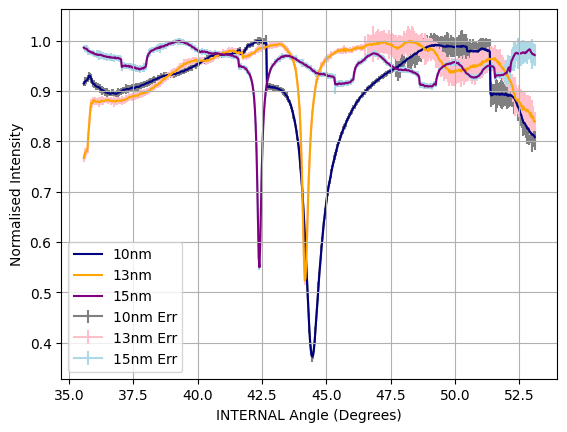
\includegraphics[width=0.85\columnwidth]{redThicknessVariation.png}
				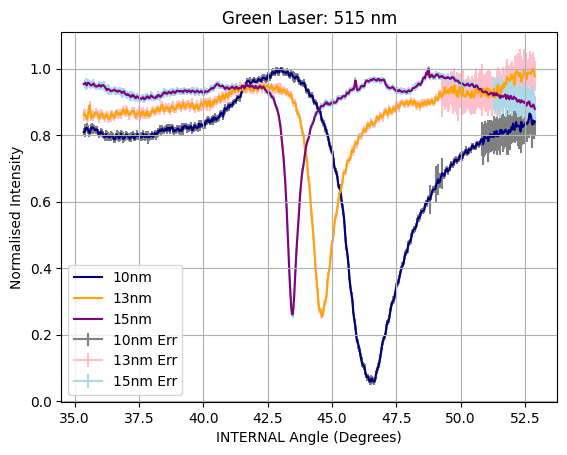
\includegraphics[width=0.85\columnwidth]{greenThicknessVariation.png}
				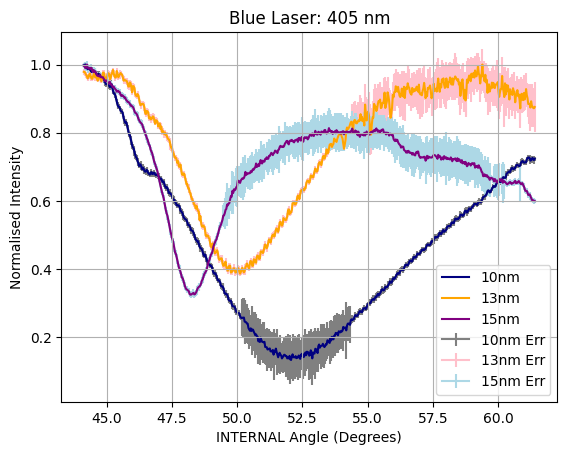
\includegraphics[width=0.85\columnwidth]{blueThicknessVariation.png}
				\caption{\label{fig:thicknessVariation}Plots visualising the variation between each film thickness across all three wavelengths. A thickness dependence of the excitation angle can clearly be visually seen as the minima consistently move towards smaller internal angles as the thickness increases. There appears to be some effect of the film thickness on the coupling as the extent of the extinction varies, however across the dataset no clear correlation can be made.}
			\end{figure}
	
		\subsection{Anomaly found during Red Laser Runs}
			When taking data with the red laser and unexpected result occurred. Large oscillations with a relative intensity amplitude of approximately $0.1$ could be seen in the data. This is shown as the light blue line in figure \ref{fig:oscillationsExample}. After attempting to troubleshoot any potential interferences with the data the anomaly seemed unavoidable and a workflow was developed to average multiple data runs together to eliminate the oscillations by destructive interference. This proved to be successful however after making several consecutive measurements a pattern was apparent from the data. With each consecutive measurement the period of the oscillations was increasing until, after around eight consecutive measurements ($\approx$30 minutes) the period was long enough that the change in intensity was negligible. This change in period is shown in figure \ref{fig:oscillationsExample}.\\
			
			\begin{figure}
				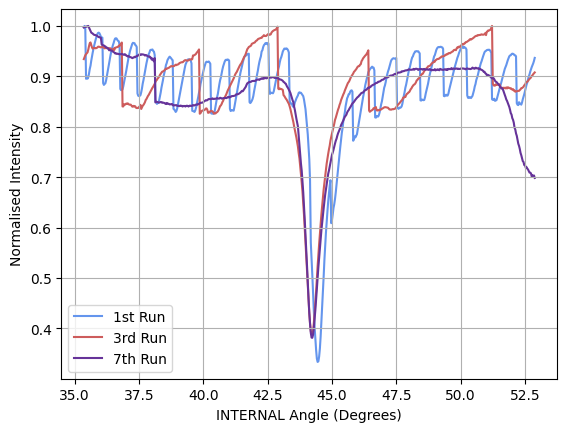
\includegraphics[width=0.85\columnwidth]{oscillationsExample.png}
				\caption{\label{fig:oscillationsExample}An example measurement showing the oscillations apparent in the red laser measurements. Consecutive measurements were taken. This plot displays the 1st, 3rd, and 7th runs showing the apparent change in the oscillations over time. In the 7th run, the oscillations are barely apparent and would not be noticed as such if not for the data taken prior.}
			\end{figure}
			
			E. R. Jones describes varying intensity from helium-neon lasers after the light is passed through a linear polariser during an approximately hour long warm-up period after a cold start \cite{jonesPolarisation}. He describes the cause of the effect to be from a few factors: The width of the lasing transition line, the resonant frequencies of the cavity between the mirrors, and the thermal expansion of the laser tube. The figures in this paper and another by Woolsey et al. \cite{woolseyPolarisation} closely match the change in the period of oscillations over time as shown in figure \ref{fig:stillData}. It is important to note that this effect was noticed in the other lasers too but to a much lesser, and in most cases, a negligible effect. This leads us to believe that this laser in particular has become somewhat defective with use.
			
			\begin{figure}
				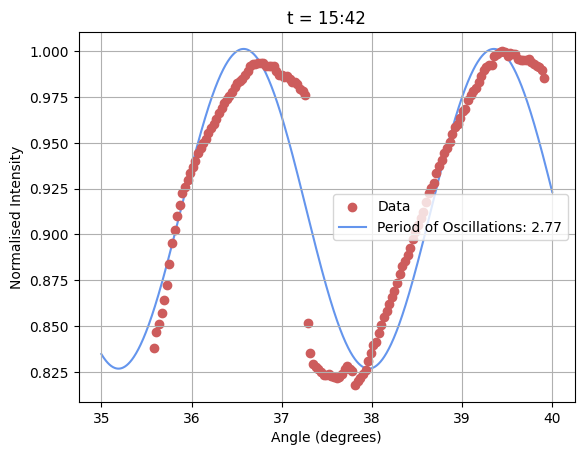
\includegraphics[width=0.85\columnwidth]{exampleTimeDependence.png}
				\caption{\label{fig:exampleTimeDependence}An example of how the oscillations in the data closely resemble a sinusoidal wave. This is a sample taken from a standard run of the data collection algorithm approximately 18 minutes after the laser was turned on and started warming up. The period of the sin wave is noted in the legend in degrees.}
			\end{figure}
			\begin{figure}
				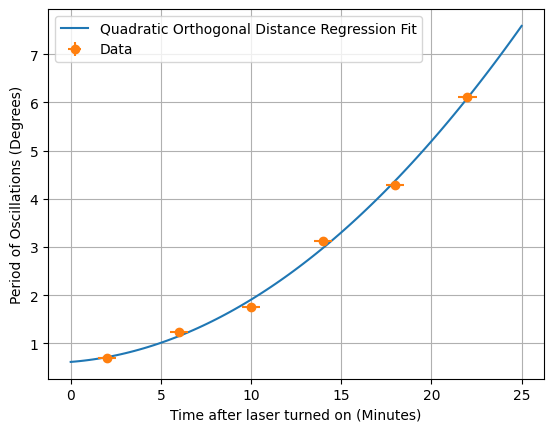
\includegraphics[width=0.85\columnwidth]{quadraticFit.png}
				\caption{\label{fig:quadraticDependence}The quadratic orthogonal distance regression fit of the period of oscillations against the time after the laser was turned on. Following this quadratic curve upwards of thirty seconds the period becomes large enough as to be greater than the range in which the data collection is being carried out.}
			\end{figure}
			\begin{figure}
				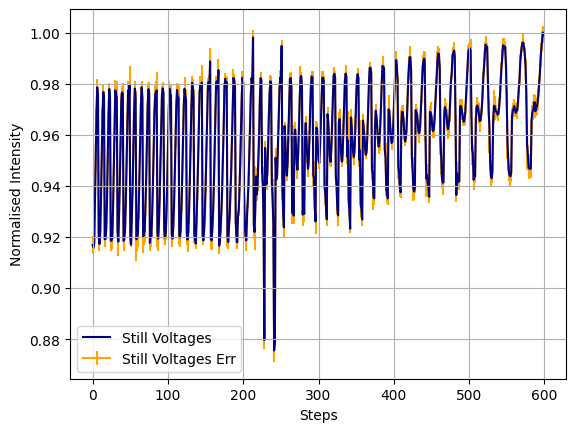
\includegraphics[width=0.85\columnwidth]{stillData.png}
				\caption{\label{fig:stillData}Data taken where the red laser is directly incident on the detector and without the motors turning. The oscillations are still present in this case and can visibly be seen to increase in period over time. Note that although the x axis is represented as steps, these are irrelevant of motor turning and instead mark steps of approximately 0.3 seconds delays between measurements for a full time frame of 3 minutes. The increase in average intensity towards the later part of the plot is unknown but is likely also a part of the "warm-up" process of helium-neon lasers.}
			\end{figure}

	\section{Conclusion}
		
		
	\clearpage
	\bibliography{surfacePlasmons}% Produces the bibliography via BibTeX.
		
	\clearpage
	\appendix
		
	\section{Python Code}
	
		\subsection{Data Acquisition}
		
		\subsection{Analysis}
		
\end{document}

